% ═══════════════════════════════════════════════════════════════════════════════
%  AI Exam Correcting System — Rapport de Projet
%  Hybrid BERT + LLM Architecture for Automated Short Answer Grading
%  École Supérieure des Communications de Tunis
% ═══════════════════════════════════════════════════════════════════════════════

\documentclass[12pt, a4paper]{report}

% ── Packages ──────────────────────────────────────────────────────────────────
\usepackage[utf8]{inputenc}
\usepackage[T1]{fontenc}
\usepackage[english]{babel}
\usepackage{geometry}
\geometry{margin=2.5cm, top=2.5cm, bottom=2.5cm}

\usepackage{graphicx}
\usepackage{xcolor}
\usepackage{titlesec}
\usepackage{titletoc}
\usepackage{fancyhdr}
\usepackage{hyperref}
\usepackage{amsmath, amssymb}
\usepackage{algorithm}
\usepackage{algpseudocode}
\usepackage{booktabs}
\usepackage{tabularx}
\usepackage{longtable}
\usepackage{multirow}
\usepackage{enumitem}
\usepackage{listings}
\usepackage{tcolorbox}
\usepackage{tikz}
\usepackage{pgfplots}
\pgfplotsset{compat=1.18}
\usetikzlibrary{shapes.geometric, arrows.meta, positioning, calc, decorations.pathreplacing, fit, backgrounds}
\usepackage{float}
\usepackage{caption}
\usepackage{subcaption}
\usepackage{setspace}
\usepackage{parskip}
\usepackage{pdfpages}
\usepackage{fontawesome5}
\usepackage{tocloft}

\tcbuselibrary{skins, breakable, listings}

% ── Colors ────────────────────────────────────────────────────────────────────
\definecolor{supcomblue}{RGB}{0, 51, 102}
\definecolor{supcomdark}{RGB}{15, 23, 42}
\definecolor{accentpurple}{RGB}{99, 102, 241}
\definecolor{accentviolet}{RGB}{139, 92, 246}
\definecolor{codegreen}{RGB}{52, 211, 153}
\definecolor{codegray}{RGB}{148, 163, 184}
\definecolor{codebg}{RGB}{15, 23, 42}
\definecolor{lightbg}{RGB}{241, 245, 249}
\definecolor{warnred}{RGB}{248, 113, 113}

% ── Hyperref setup ────────────────────────────────────────────────────────────
\hypersetup{
    colorlinks=true,
    linkcolor=supcomblue,
    citecolor=accentpurple,
    urlcolor=accentviolet,
    pdftitle={AI Exam Correcting System - Hybrid BERT + LLM Architecture},
    pdfauthor={Khalifa Bouneb, Ines Jebri, Marwen Boussabbat},
}

% ── Code listing style ────────────────────────────────────────────────────────
\lstdefinestyle{pythonstyle}{
    language=Python,
    basicstyle=\ttfamily\small,
    keywordstyle=\color{accentpurple}\bfseries,
    stringstyle=\color{codegreen},
    commentstyle=\color{codegray}\itshape,
    numberstyle=\tiny\color{codegray},
    numbers=left,
    numbersep=8pt,
    backgroundcolor=\color{lightbg},
    frame=single,
    rulecolor=\color{codegray!30},
    breaklines=true,
    breakatwhitespace=true,
    tabsize=4,
    showstringspaces=false,
    captionpos=b,
    xleftmargin=1.5em,
    framexleftmargin=1.5em,
    aboveskip=1em,
    belowskip=1em,
}
\lstset{style=pythonstyle}

% ── Custom tcolorbox styles ───────────────────────────────────────────────────
\newtcolorbox{infobox}[1][]{
    colback=accentpurple!5,
    colframe=accentpurple!60,
    fonttitle=\bfseries,
    title=#1,
    arc=3pt,
    boxrule=0.8pt,
    left=8pt, right=8pt,
    top=6pt, bottom=6pt,
    breakable,
}

\newtcolorbox{formulabox}[1][]{
    colback=supcomblue!3,
    colframe=supcomblue!50,
    fonttitle=\bfseries,
    title=#1,
    arc=3pt,
    boxrule=0.8pt,
    left=8pt, right=8pt,
    top=6pt, bottom=6pt,
}

% ── Chapter and section formatting ────────────────────────────────────────────
\titleformat{\chapter}[display]
    {\normalfont\huge\bfseries\color{supcomblue}}
    {\chaptertitlename\ \thechapter}{20pt}{\Huge}
\titlespacing*{\chapter}{0pt}{-20pt}{30pt}

\titleformat{\section}
    {\normalfont\Large\bfseries\color{supcomblue!90}}
    {\thesection}{1em}{}
\titleformat{\subsection}
    {\normalfont\large\bfseries\color{supcomblue!75}}
    {\thesubsection}{1em}{}
\titleformat{\subsubsection}
    {\normalfont\normalsize\bfseries\color{supcomblue!60}}
    {\thesubsubsection}{1em}{}

% ── Header and footer ────────────────────────────────────────────────────────
\pagestyle{fancy}
\fancyhf{}
\fancyhead[L]{\small\color{codegray}\leftmark}
\fancyhead[R]{\small\color{codegray}AI Exam Correcting System}
\fancyfoot[C]{\thepage}
\renewcommand{\headrulewidth}{0.4pt}
\renewcommand{\footrulewidth}{0pt}

% ── Line spacing ──────────────────────────────────────────────────────────────
\setstretch{1.3}

% ═══════════════════════════════════════════════════════════════════════════════
%  DOCUMENT START
% ═══════════════════════════════════════════════════════════════════════════════
\begin{document}

% ══════════════════════════════════════════════════════════════════════════════
%  PAGE DE GARDE
% ══════════════════════════════════════════════════════════════════════════════
\begin{titlepage}
\begin{tikzpicture}[remember picture, overlay]

    % ── White background ──────────────────────────────────────────────────
    \fill[white] (current page.south west) rectangle (current page.north east);

    % ── Single navy blue bar at top ───────────────────────────────────────
    \fill[supcomblue] 
        (current page.north west) rectangle ([yshift=-3.5cm]current page.north east);

    % ── Republic & Ministry (white on navy) ───────────────────────────────
    \node[anchor=north, text=white, font=\fontsize{11}{13}\selectfont]
        at ([yshift=-0.8cm]current page.north) {
        \textsc{R\'{e}publique Tunisienne}
    };
    \node[anchor=north, text=white!80, font=\fontsize{9}{11}\selectfont]
        at ([yshift=-1.4cm]current page.north) {
        Minist\`{e}re des Technologies de la Communication
    };

    % ── Thin gold/accent separator inside the bar ─────────────────────────
    \draw[accentpurple, line width=0.6pt]
        ([yshift=-1.85cm, xshift=3cm]current page.north west) --
        ([yshift=-1.85cm, xshift=-3cm]current page.north east);

    % ── University name (white on navy) ───────────────────────────────────
    \node[anchor=north, text=white, font=\fontsize{15}{18}\selectfont\bfseries,
          text width=14cm, align=center]
        at ([yshift=-2.15cm]current page.north) {
        \'{E}cole Sup\'{e}rieure des Communications de Tunis
    };
    \node[anchor=north, text=white!70, font=\fontsize{8}{10}\selectfont\ttfamily\bfseries]
        at ([yshift=-3.0cm]current page.north) {
        SUP'COM
    };

    % ── Thin accent line below the bar ────────────────────────────────────
    \fill[accentpurple] 
        ([yshift=-3.5cm]current page.north west) rectangle ([yshift=-3.58cm]current page.north east);

    % ══════════════════════════════════════════════════════════════════════
    %  CENTER — Title area (dark text on white)
    % ══════════════════════════════════════════════════════════════════════

    % Subject / course
    \node[anchor=center, text=supcomblue!70, font=\fontsize{11}{13}\selectfont\itshape]
        at ([yshift=5.5cm]current page.center) {
        Optimisation et M\'{e}ta-heuristiques
    };

    % Small rule
    \draw[supcomblue, line width=0.4pt]
        ([yshift=5.0cm, xshift=-2cm]current page.center) --
        ([yshift=5.0cm, xshift=2cm]current page.center);

    % Main title
    \node[anchor=center, text=supcomblue, 
          font=\fontsize{30}{36}\selectfont\bfseries,
          text width=14cm, align=center]
        at ([yshift=3.2cm]current page.center) {
        AI Exam Correcting\\System
    };

    % Subtitle
    \node[anchor=center, text=supcomblue!65,
          font=\fontsize{13}{17}\selectfont,
          text width=14cm, align=center]
        at ([yshift=1.5cm]current page.center) {
        Hybrid BERT + LLM Architecture for\\[2pt]
        Automated Short Answer Grading
    };

    % Accent underline
    \draw[accentpurple, line width=2pt]
        ([yshift=0.7cm, xshift=-3cm]current page.center) --
        ([yshift=0.7cm, xshift=3cm]current page.center);

    % ══════════════════════════════════════════════════════════════════════
    %  LOWER — Authors & Supervisor (clean table style)
    % ══════════════════════════════════════════════════════════════════════

    % Box frame
    \draw[supcomblue!30, line width=0.6pt, rounded corners=6pt]
        ([xshift=2.5cm, yshift=-1.0cm]current page.center) rectangle
        ([xshift=-2.5cm, yshift=-4.8cm]current page.center);

    % Left column header
    \node[anchor=north west, text=supcomblue, 
          font=\fontsize{9}{11}\selectfont\scshape\bfseries]
        at ([xshift=-6cm, yshift=-1.3cm]current page.center) {
        Prepared by
    };
    % Left column names
    \node[anchor=north west, text=black!80,
          font=\fontsize{11}{15}\selectfont]
        at ([xshift=-6cm, yshift=-1.9cm]current page.center) {
        \begin{tabular}{@{}l@{}}
            Khalifa Bouneb\\[3pt]
            Ines Jebri\\[3pt]
            Marwen Boussabbat
        \end{tabular}
    };

    % Vertical separator
    \draw[supcomblue!20, line width=0.4pt]
        ([yshift=-1.15cm]current page.center) -- ([yshift=-4.65cm]current page.center);

    % Right column header
    \node[anchor=north west, text=supcomblue,
          font=\fontsize{9}{11}\selectfont\scshape\bfseries]
        at ([xshift=0.8cm, yshift=-1.3cm]current page.center) {
        Supervised by
    };
    % Right column name
    \node[anchor=north west, text=black!80,
          font=\fontsize{11}{15}\selectfont]
        at ([xshift=0.8cm, yshift=-1.9cm]current page.center) {
        \begin{tabular}{@{}l@{}}
            Jaleleddine Ben Amor\\[3pt]
            {\small\itshape\color{supcomblue!50} SUP'COM}
        \end{tabular}
    };

    % ══════════════════════════════════════════════════════════════════════
    %  FOOTER — Navy bar at bottom
    % ══════════════════════════════════════════════════════════════════════
    \fill[supcomblue]
        (current page.south west) rectangle ([yshift=1.2cm]current page.south east);
    \fill[accentpurple]
        ([yshift=1.2cm]current page.south west) rectangle ([yshift=1.28cm]current page.south east);

    \node[anchor=center, text=white, font=\fontsize{10}{12}\selectfont]
        at ([yshift=0.6cm]current page.south) {
        \textsc{Academic Year 2025\,--\,2026}
    };

\end{tikzpicture}
\end{titlepage}

% ══════════════════════════════════════════════════════════════════════════════
%  TABLE OF CONTENTS
% ══════════════════════════════════════════════════════════════════════════════
\pagenumbering{roman}
\tableofcontents
\newpage
\listoffigures
\listoftables
\newpage
\pagenumbering{arabic}

% ══════════════════════════════════════════════════════════════════════════════
%  CHAPTER 1 — INTRODUCTION
% ══════════════════════════════════════════════════════════════════════════════
\chapter{Introduction}

\section{Context and Motivation}

The assessment of student exam responses remains one of the most time-consuming tasks in education. Instructors spend countless hours manually grading short-answer questions, where evaluating the semantic correctness of each response against a reference answer requires deep reading and expert judgement. As class sizes grow and the demand for timely feedback intensifies, \textbf{Automated Short Answer Grading (ASAG)} has emerged as a critical research area at the intersection of \textbf{Natural Language Processing (NLP)}, \textbf{Computer Vision (CV)}, and \textbf{Artificial Intelligence (AI)}.

Traditional automated grading systems rely on keyword matching or rule-based approaches, which fail to capture the rich semantic nuances of natural language. Two complementary paradigms have shown significant promise in recent years:

\begin{enumerate}[leftmargin=2em]
    \item \textbf{Embedding-based semantic similarity} — Transformer models like BERT encode text into dense vector representations where cosine similarity directly measures meaning overlap.
    \item \textbf{Large Language Model (LLM) reasoning} — Modern LLMs can understand context, detect factual errors, award partial credit, and generate constructive feedback.
\end{enumerate}

Neither approach is perfect in isolation. BERT embeddings provide fast, deterministic similarity scores but lack interpretive reasoning. LLMs offer nuanced judgement and feedback but can be inconsistent and expensive. This motivates our \textbf{hybrid approach}.

\section{Project Objectives}

This project implements a complete, end-to-end AI-powered exam correction pipeline with the following objectives:

\begin{itemize}[leftmargin=2em]
    \item \textbf{OCR-based input}: Accept exam papers as images or PDFs and extract student answers using Optical Character Recognition.
    \item \textbf{Semantic scoring via BERT}: Compute embedding-based similarity between student and reference answers.
    \item \textbf{LLM-based intelligent grading}: Leverage a Large Language Model to assign nuanced scores with constructive feedback.
    \item \textbf{Hybrid scoring formula}: Combine both approaches via an optimisable blending parameter $\alpha$.
    \item \textbf{Dataset evaluation}: Validate the pipeline against standard ASAG benchmarks with rigorous metrics.
    \item \textbf{User-friendly interface}: Provide an intuitive Streamlit web application for teachers.
\end{itemize}

\section{Report Structure}

This report is organised as follows:

\begin{itemize}[leftmargin=2em]
    \item \textbf{Chapter 2} — Literature review and theoretical background on BERT, LLMs, OCR, and ASAG.
    \item \textbf{Chapter 3} — System architecture and detailed design of each module.
    \item \textbf{Chapter 4} — Implementation details, code structure, and technology stack.
    \item \textbf{Chapter 5} — Hybrid scoring optimisation and the role of meta-heuristics.
    \item \textbf{Chapter 6} — Experimental evaluation, datasets, and results.
    \item \textbf{Chapter 7} — User interface design and demonstration.
    \item \textbf{Chapter 8} — Conclusion and future work.
\end{itemize}


% ══════════════════════════════════════════════════════════════════════════════
%  CHAPTER 2 — THEORETICAL BACKGROUND
% ══════════════════════════════════════════════════════════════════════════════
\chapter{Theoretical Background}

\section{Automated Short Answer Grading (ASAG)}

Automated Short Answer Grading is the task of computationally assessing free-text student responses against a reference answer. Unlike multiple-choice questions, short answers exhibit high variability in phrasing, length, and structure while potentially conveying equivalent semantic meaning.

\subsection{Historical Approaches}

ASAG research has evolved through several generations:

\begin{table}[H]
\centering
\caption{Evolution of ASAG approaches}
\label{tab:asag_history}
\begin{tabularx}{\textwidth}{lXl}
\toprule
\textbf{Era} & \textbf{Approach} & \textbf{Limitation} \\
\midrule
1960s--1990s & Keyword matching, pattern rules & No semantic understanding \\
2000s & TF-IDF, LSA, WordNet similarity & Shallow semantics \\
2010s & Word2Vec, GloVe embeddings & Context-independent \\
2018+ & BERT, Transformer encoders & Deterministic, no reasoning \\
2023+ & LLMs (GPT, LLaMA, Gemini) & Costly, non-deterministic \\
\midrule
\textbf{Ours} & \textbf{Hybrid BERT + LLM} & \textbf{Best of both worlds} \\
\bottomrule
\end{tabularx}
\end{table}

\subsection{Key Challenges in ASAG}

\begin{enumerate}[leftmargin=2em]
    \item \textbf{Semantic equivalence}: ``Plants use sunlight to make food'' $\equiv$ ``Photosynthesis converts light energy into chemical energy'' — same meaning, completely different words.
    \item \textbf{Partial credit}: Answers may be partially correct, requiring graded scoring rather than binary classification.
    \item \textbf{Factual accuracy}: An answer may be semantically similar but factually wrong.
    \item \textbf{Domain generality}: The system must work across subjects (biology, physics, computer science, etc.).
\end{enumerate}

\section{BERT and Sentence Transformers}

\subsection{BERT Architecture}

BERT (Bidirectional Encoder Representations from Transformers), introduced by Devlin et al. (2019), is a transformer-based pre-trained language model. Unlike previous models that read text unidirectionally, BERT processes the entire sequence simultaneously through \textbf{multi-head self-attention}:

\begin{formulabox}[Self-Attention Mechanism]
\begin{equation}
    \text{Attention}(Q, K, V) = \text{softmax}\left(\frac{QK^T}{\sqrt{d_k}}\right) V
    \label{eq:attention}
\end{equation}
where $Q$, $K$, $V$ are query, key, and value matrices projected from the input embeddings, and $d_k$ is the dimension of the key vectors.
\end{formulabox}

The model is pre-trained on two objectives:
\begin{itemize}[leftmargin=2em]
    \item \textbf{Masked Language Modelling (MLM)}: Predict randomly masked tokens from context.
    \item \textbf{Next Sentence Prediction (NSP)}: Determine if two sentences are consecutive.
\end{itemize}

\subsection{Sentence-Transformers and Cosine Similarity}

Standard BERT produces token-level embeddings. For sentence-level comparison, \textbf{Sentence-Transformers} (Reimers \& Gurevych, 2019) fine-tune BERT using a Siamese architecture on Semantic Textual Similarity (STS) datasets, producing fixed-size sentence embeddings where geometric distance reflects semantic distance.

\begin{formulabox}[Cosine Similarity]
\begin{equation}
    \text{cos\_sim}(\mathbf{u}, \mathbf{v}) = \frac{\mathbf{u} \cdot \mathbf{v}}{\|\mathbf{u}\| \cdot \|\mathbf{v}\|} \in [-1, 1]
    \label{eq:cosine}
\end{equation}
For L2-normalised embeddings (as used in our system), this simplifies to the dot product: $\text{cos\_sim}(\hat{\mathbf{u}}, \hat{\mathbf{v}}) = \hat{\mathbf{u}} \cdot \hat{\mathbf{v}}$.
\end{formulabox}

In our system, we use the \texttt{all-MiniLM-L6-v2} model:
\begin{itemize}[leftmargin=2em]
    \item 6 transformer layers, 384-dimensional output embeddings
    \item Trained on over 1 billion sentence pairs
    \item Max sequence length: 256 tokens
    \item Fast inference ($\sim$5ms per sentence on CPU)
\end{itemize}

\subsection{From Similarity to Score}

The cosine similarity $c \in [0, 1]$ is linearly mapped to the grading scale:
\begin{equation}
    S_{\text{BERT}} = \max\left(0,\; \min\left(M,\; c \times M\right)\right)
    \label{eq:bert_score}
\end{equation}
where $M$ is the maximum score for the question.

\section{Large Language Models (LLMs)}

\subsection{Architecture and Capabilities}

Large Language Models are autoregressive transformers trained on massive text corpora. Models like LLaMA-3.3-70B (Meta, 2024) demonstrate:
\begin{itemize}[leftmargin=2em]
    \item \textbf{Contextual reasoning}: Understanding question context and evaluating factual correctness.
    \item \textbf{Partial credit assessment}: Recognising partially correct responses.
    \item \textbf{Feedback generation}: Producing constructive explanations.
    \item \textbf{Rubric adherence}: Following structured grading criteria when prompted.
\end{itemize}

\subsection{Prompt Engineering for Grading}

We design a structured system prompt that instructs the LLM to:
\begin{enumerate}[leftmargin=2em]
    \item Use the BERT cosine similarity as a \textit{semantic baseline}.
    \item Apply expert judgement on top of the baseline.
    \item Reward correct key concepts even if phrased differently.
    \item Penalise factual errors and missing critical points.
    \item Return a structured JSON response with score and feedback.
\end{enumerate}

\subsection{API Providers}

Our system supports three free LLM API providers for flexibility:

\begin{table}[H]
\centering
\caption{Supported LLM providers}
\label{tab:llm_providers}
\begin{tabular}{llll}
\toprule
\textbf{Provider} & \textbf{Model} & \textbf{Parameters} & \textbf{Free Tier} \\
\midrule
Groq & LLaMA-3.3-70B-Versatile & 70B & Yes \\
Google & Gemini 2.0 Flash & --- & Yes \\
OpenRouter & LLaMA-3.3-70B-Instruct & 70B & Yes \\
\bottomrule
\end{tabular}
\end{table}

\section{Optical Character Recognition (OCR)}

\subsection{EasyOCR Engine}

EasyOCR is an open-source OCR library supporting 80+ languages. It uses a two-stage pipeline:
\begin{enumerate}[leftmargin=2em]
    \item \textbf{Text Detection}: CRAFT (Character Region Awareness for Text detection) neural network localises text regions.
    \item \textbf{Text Recognition}: A CRNN (Convolutional Recurrent Neural Network) with CTC (Connectionist Temporal Classification) decoding transcribes detected regions.
\end{enumerate}

\subsection{Image Preprocessing with OpenCV}

To improve OCR accuracy on real-world exam scans, we apply preprocessing:
\begin{enumerate}[leftmargin=2em]
    \item \textbf{Grayscale conversion}: Reduce 3-channel RGB to single-channel intensity.
    \item \textbf{Adaptive thresholding}: Binarise the image using a Gaussian-weighted local threshold, robust to uneven lighting:
    \begin{equation}
        T(x, y) = \text{mean}_{w \times w}\bigl(I(x, y)\bigr) - C
    \end{equation}
    where $w = 31$ is the block size and $C = 10$ is the constant subtracted from the mean.
\end{enumerate}

\subsection{PDF Text Extraction}

For digital (typed) PDFs, we use \textbf{PyMuPDF} to extract embedded text directly — this is instant and avoids OCR entirely. For scanned PDFs, pages are rendered to images at 150 DPI, then processed through the OCR pipeline.


% ══════════════════════════════════════════════════════════════════════════════
%  CHAPTER 3 — SYSTEM ARCHITECTURE
% ══════════════════════════════════════════════════════════════════════════════
\chapter{System Architecture}

\section{High-Level Overview}

The system follows a modular pipeline architecture. Each component is an independent Python module with a well-defined API, enabling easy testing, replacement, and extension.

\begin{figure}[H]
\centering
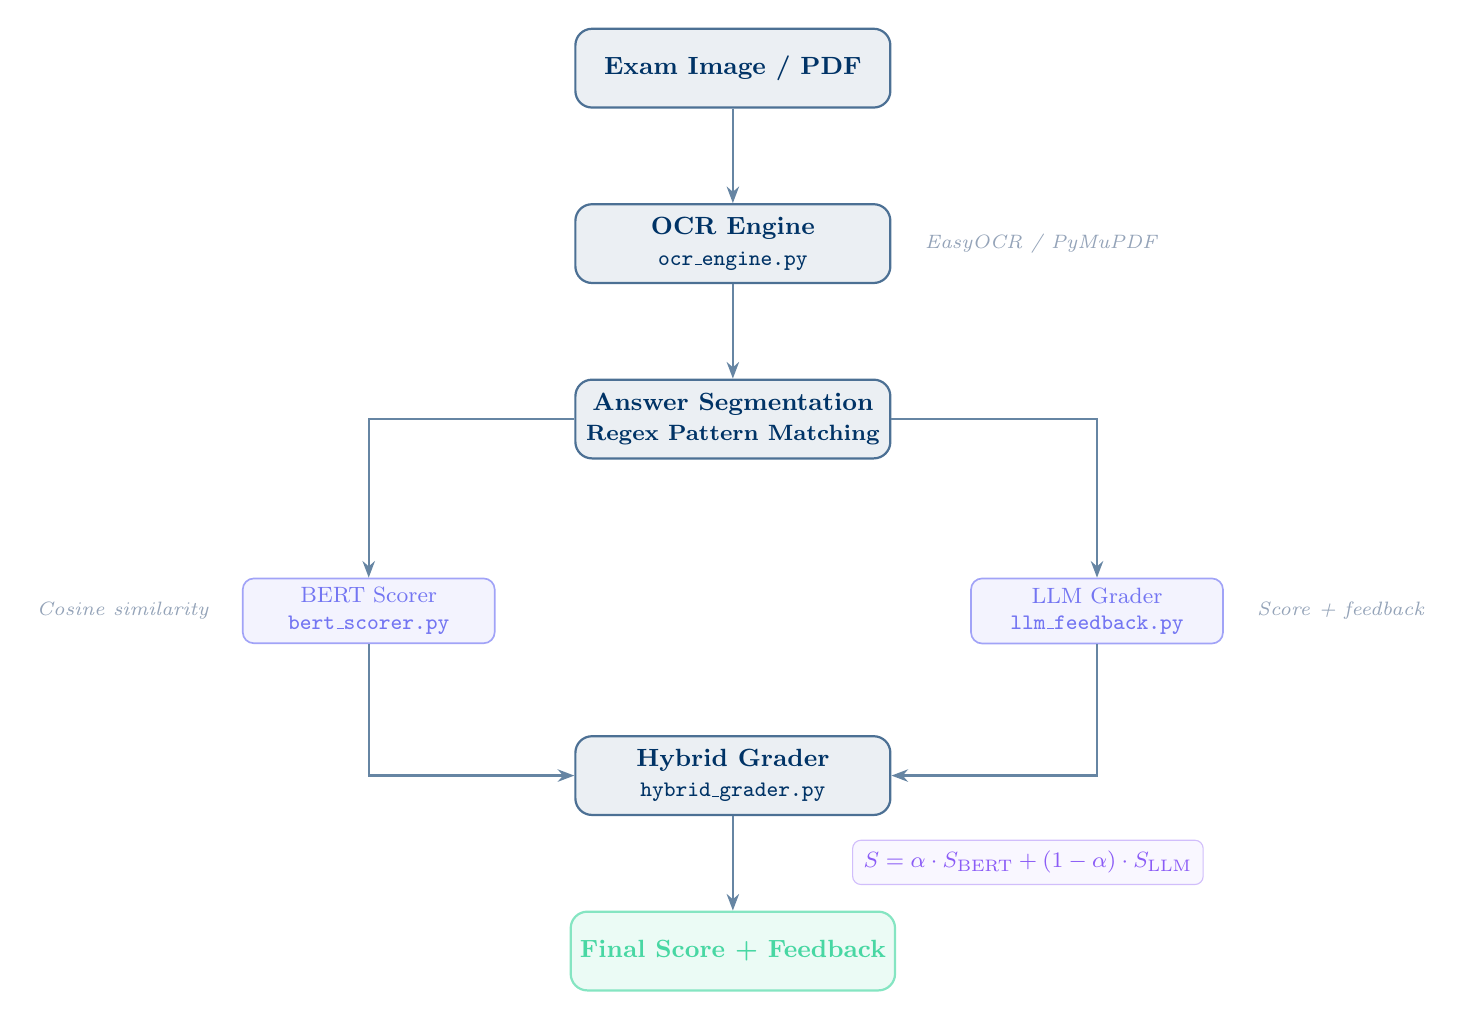
\begin{tikzpicture}[
    node distance=1.2cm and 2cm,
    box/.style={draw=supcomblue!70, fill=supcomblue!8, rounded corners=6pt, 
                minimum width=4cm, minimum height=1cm, font=\small\bfseries,
                text=supcomblue, align=center, line width=0.8pt},
    smallbox/.style={draw=accentpurple!60, fill=accentpurple!8, rounded corners=4pt,
                     minimum width=3.2cm, minimum height=0.8cm, font=\footnotesize,
                     text=accentpurple!90, align=center, line width=0.6pt},
    arrow/.style={-{Stealth[length=6pt]}, line width=0.8pt, color=supcomblue!60},
    dasharrow/.style={-{Stealth[length=5pt]}, line width=0.6pt, dashed, color=codegray},
]
    % Main pipeline
    \node[box] (input) {Exam Image / PDF};
    \node[box, below=of input] (ocr) {OCR Engine\\{\footnotesize\texttt{ocr\_engine.py}}};
    \node[box, below=of ocr] (segment) {Answer Segmentation\\{\footnotesize Regex Pattern Matching}};
    
    % Parallel scoring
    \node[smallbox, below left=1.5cm and 1cm of segment] (bert) {BERT Scorer\\{\footnotesize\texttt{bert\_scorer.py}}};
    \node[smallbox, below right=1.5cm and 1cm of segment] (llm) {LLM Grader\\{\footnotesize\texttt{llm\_feedback.py}}};
    
    % Hybrid
    \node[box, below=3.5cm of segment] (hybrid) {Hybrid Grader\\{\footnotesize\texttt{hybrid\_grader.py}}};
    
    % Output
    \node[box, below=of hybrid, fill=codegreen!10, draw=codegreen!60, text=codegreen!90] (output) {Final Score + Feedback};
    
    % Arrows
    \draw[arrow] (input) -- (ocr);
    \draw[arrow] (ocr) -- (segment);
    \draw[arrow] (segment) -| (bert);
    \draw[arrow] (segment) -| (llm);
    \draw[arrow] (bert) |- (hybrid);
    \draw[arrow] (llm) |- (hybrid);
    \draw[arrow] (hybrid) -- (output);
    
    % Side annotations
    \node[font=\scriptsize\itshape, text=codegray, right=0.3cm of ocr] {EasyOCR / PyMuPDF};
    \node[font=\scriptsize\itshape, text=codegray, left=0.3cm of bert] {Cosine similarity};
    \node[font=\scriptsize\itshape, text=codegray, right=0.3cm of llm] {Score + feedback};
    
    % Formula box
    \node[draw=accentviolet!40, fill=accentviolet!5, rounded corners=3pt, 
          font=\footnotesize, text=accentviolet, inner sep=4pt,
          below right=0.3cm and -0.5cm of hybrid] {
        $S = \alpha \cdot S_{\text{BERT}} + (1-\alpha) \cdot S_{\text{LLM}}$
    };
\end{tikzpicture}
\caption{Complete system architecture — hybrid BERT + LLM grading pipeline}
\label{fig:architecture}
\end{figure}

\section{Module Descriptions}

\subsection{Configuration Module (\texttt{config.py})}

Centralises all configurable parameters using environment variables loaded from a \texttt{.env} file. This ensures:
\begin{itemize}[leftmargin=2em]
    \item \textbf{Security}: API keys are never hardcoded.
    \item \textbf{Flexibility}: Parameters can be changed without modifying code.
    \item \textbf{Reproducibility}: The \texttt{.env} file documents the exact configuration used.
\end{itemize}

Key configuration parameters:

\begin{table}[H]
\centering
\caption{System configuration parameters}
\label{tab:config}
\begin{tabularx}{\textwidth}{lXl}
\toprule
\textbf{Parameter} & \textbf{Description} & \textbf{Default} \\
\midrule
\texttt{ALPHA} & BERT weight in hybrid formula & 0.4 \\
\texttt{BERT\_MODEL\_NAME} & Sentence-Transformers model & \texttt{all-MiniLM-L6-v2} \\
\texttt{LLM\_PROVIDER} & Active LLM API provider & \texttt{groq} \\
\texttt{LLM\_TEMPERATURE} & LLM generation temperature & 0.2 \\
\texttt{OCR\_ENGINE} & OCR backend & \texttt{easyocr} \\
\texttt{OCR\_LANGUAGES} & OCR language list & \texttt{en, fr} \\
\texttt{MAX\_SCORE} & Default max score per question & 20 \\
\bottomrule
\end{tabularx}
\end{table}

\subsection{OCR Engine (\texttt{ocr\_engine.py})}

The OCR module handles the full pipeline from file input to structured text:

\begin{enumerate}[leftmargin=2em]
    \item \textbf{Input handling}: Supports PNG, JPG, BMP, TIFF images and PDF files.
    \item \textbf{PDF optimisation}: For digital PDFs, text is extracted natively via PyMuPDF (instant). Scanned PDFs are rendered to images at 150 DPI.
    \item \textbf{Preprocessing}: OpenCV adaptive thresholding for improved OCR accuracy.
    \item \textbf{Text extraction}: EasyOCR processes the image and returns raw text.
    \item \textbf{Answer segmentation}: Regex patterns detect question markers (\texttt{Q1:}, \texttt{1.}, \texttt{1)}, etc.) and split the text into individual answers.
\end{enumerate}

\begin{lstlisting}[caption={Answer segmentation regex pattern}, label={lst:regex}]
# Pattern: number (optionally preceded by Q/Question) 
# followed by separator
pattern = r'(?:^|\n)\s*(?:Q(?:uestion)?\s*)?(\d+)\s*[).::\-]\s*'
splits = re.split(pattern, raw_text, flags=re.IGNORECASE)
\end{lstlisting}

\subsection{BERT Scorer (\texttt{bert\_scorer.py})}

This module provides semantic similarity scoring:

\begin{enumerate}[leftmargin=2em]
    \item \textbf{Model loading}: Lazy initialisation of the sentence-transformers model (cached for process lifetime).
    \item \textbf{Encoding}: Both reference and student answers are encoded into L2-normalised 384-dimensional vectors.
    \item \textbf{Similarity}: Cosine similarity is computed as the dot product of normalised embeddings.
    \item \textbf{Score mapping}: The similarity $\in [0, 1]$ is linearly scaled to $[0, M]$.
\end{enumerate}

\begin{lstlisting}[caption={BERT scoring core logic}, label={lst:bert_score}]
def score(reference: str, student: str, max_score: float) -> BERTScoreResult:
    emb = encode([reference, student])  # L2-normalised
    cos_sim = cosine_similarity(emb[0], emb[1])
    clamped = max(0.0, min(1.0, cos_sim))
    normalised = round(clamped * max_score, 2)
    return BERTScoreResult(
        cosine_similarity=cos_sim,
        normalised_score=normalised,
        max_score=max_score,
    )
\end{lstlisting}

\subsection{LLM Feedback (\texttt{llm\_feedback.py})}

The LLM grading module:

\begin{enumerate}[leftmargin=2em]
    \item \textbf{Prompt construction}: Builds a structured system prompt that instructs the LLM to grade using a specific rubric and return JSON.
    \item \textbf{API call}: Sends the reference answer, student answer, and BERT cosine similarity to one of three supported providers.
    \item \textbf{Response parsing}: Extracts the score and feedback from the JSON response, with a regex fallback for robustness.
    \item \textbf{Error handling}: Graceful degradation with retry and response cleaning.
\end{enumerate}

Key design decision: the \textbf{BERT cosine similarity is passed to the LLM as context}. This allows the LLM to calibrate its score relative to the embedding similarity, producing more consistent grades:

\begin{lstlisting}[caption={LLM user message template (simplified)}, label={lst:llm_prompt}]
Reference Answer: "{reference}"
Student Answer: "{student}"
Cosine Similarity: {cosine_sim:.4f}  (0 = unrelated, 1 = identical)

Grade the student's answer. Return JSON: {"score": <num>, "feedback": "<text>"}
\end{lstlisting}

\subsection{Hybrid Grader (\texttt{hybrid\_grader.py})}

The central module that orchestrates the full pipeline for each question:

\begin{formulabox}[Hybrid Scoring Formula]
\begin{equation}
    S_{\text{final}} = \alpha \cdot S_{\text{BERT}} + (1 - \alpha) \cdot S_{\text{LLM}}
    \label{eq:hybrid}
\end{equation}
where:
\begin{itemize}[leftmargin=2em]
    \item $S_{\text{BERT}}$: BERT-based normalised score $\in [0, M]$
    \item $S_{\text{LLM}}$: LLM-assigned score $\in [0, M]$
    \item $\alpha \in [0, 1]$: Blending weight (default 0.4, configurable)
    \item $M$: Maximum score for the question
\end{itemize}
The final score is clamped to $[0, M]$.
\end{formulabox}

The module provides:
\begin{itemize}[leftmargin=2em]
    \item \texttt{grade\_answer()}: Grade a single student answer.
    \item \texttt{grade\_exam()}: Grade a batch of question-answer pairs.
    \item \texttt{exam\_summary()}: Compute aggregate statistics (total, percentage, per-question breakdown).
    \item \texttt{HybridGradingResult}: Dataclass with score, grade letter (A+, A, B, C, D, F), percentage, timing, and component breakdown.
\end{itemize}

\subsection{Exam Manager (\texttt{exam\_manager.py})}

Manages exam templates as JSON files:
\begin{itemize}[leftmargin=2em]
    \item Teachers configure reference answers \textbf{once} via the Setup page.
    \item Templates are persisted in \texttt{exams/} as JSON files.
    \item At grading time, the student just uploads their exam paper — no manual input is needed.
    \item Supports CRUD operations: create, load, list, delete.
\end{itemize}

\subsection{Dataset Loader (\texttt{dataset\_loader.py})}

Provides standardised loaders for three major ASAG benchmarks, plus a generic CSV loader. All loaders return a unified format: \texttt{(question\_id, reference, student\_answer, gold\_score, max\_score)}.


% ══════════════════════════════════════════════════════════════════════════════
%  CHAPTER 4 — IMPLEMENTATION
% ══════════════════════════════════════════════════════════════════════════════
\chapter{Implementation Details}

\section{Technology Stack}

\begin{table}[H]
\centering
\caption{Technology stack}
\label{tab:techstack}
\begin{tabularx}{\textwidth}{llX}
\toprule
\textbf{Category} & \textbf{Technology} & \textbf{Role} \\
\midrule
Language & Python 3.13 & Core development language \\
\midrule
\multirow{2}{*}{AI/NLP} & sentence-transformers & BERT embedding model \\
& Groq API (LLaMA 3.3 70B) & LLM grading \& feedback \\
\midrule
\multirow{3}{*}{CV/OCR} & EasyOCR & Optical character recognition \\
& OpenCV & Image preprocessing \\
& PyMuPDF (fitz) & Native PDF text extraction \\
\midrule
UI & Streamlit & Interactive web application \\
\midrule
Visualisation & Plotly & Charts (gauge, bar, radar) \\
\midrule
\multirow{3}{*}{Data/ML} & NumPy & Vector operations \\
& Pandas & Dataset handling \\
& SciPy & Correlation metrics \\
\midrule
Config & python-dotenv & Environment variable management \\
\bottomrule
\end{tabularx}
\end{table}

\section{Project Structure}

\begin{lstlisting}[language={}, caption={Project directory structure}, label={lst:structure}]
AI_Correcting/
|-- .env                    # API keys (git-ignored)
|-- .gitignore
|-- requirements.txt
|-- config.py               # Central configuration
|-- ocr_engine.py           # OCR + image preprocessing
|-- bert_scorer.py          # BERT embedding similarity
|-- llm_feedback.py         # LLM grading API calls
|-- hybrid_grader.py        # Alpha-blending pipeline
|-- exam_manager.py         # Exam template CRUD
|-- dataset_loader.py       # Dataset loaders + metrics
|-- app.py                  # Streamlit web interface
|-- test_pipeline.py        # End-to-end pipeline test
|-- exams/                  # Saved exam templates (JSON)
|-- datasets/               # Downloaded datasets
|-- samples/                # Sample exam images
\end{lstlisting}

\section{Key Implementation Decisions}

\subsection{Lazy Loading Strategy}

All heavy models (BERT, EasyOCR) are loaded lazily on first use and cached as module-level globals. In the Streamlit app, \texttt{@st.cache\_resource} ensures models persist across reruns:

\begin{lstlisting}[caption={Lazy model loading with Streamlit caching}, label={lst:caching}]
@st.cache_resource(show_spinner=False)
def load_bert():
    import bert_scorer
    bert_scorer._get_model()  # Force model download
    return bert_scorer
\end{lstlisting}

\subsection{PDF Dual-Path Strategy}

Instead of always running slow OCR on PDFs, we first attempt native text extraction:

\begin{lstlisting}[caption={PDF dual-path extraction}, label={lst:pdf_dual}]
def extract_text(file_path, preprocess=True):
    if ext == ".pdf":
        # Try native text extraction first (instant)
        native_text = extract_pdf_text_native(path)
        if native_text:
            return native_text
        # Fallback: OCR on rendered page images
        pages = load_pdf_pages(path, dpi=150)
        ...
\end{lstlisting}

This makes digital PDFs process \textbf{instantly} ($<$1s) instead of minutes.

\subsection{LLM Response Parsing}

The LLM response parser implements a two-tier strategy:
\begin{enumerate}[leftmargin=2em]
    \item \textbf{Primary}: Standard JSON parsing with \texttt{json.loads()}.
    \item \textbf{Fallback}: Regex-based extraction for malformed responses:
\end{enumerate}

\begin{lstlisting}[caption={Robust LLM response parsing}, label={lst:parsing}]
def _parse_response(raw: str, max_score: float) -> dict:
    try:
        obj = json.loads(cleaned)
        return {"score": obj["score"], "feedback": obj["feedback"]}
    except (json.JSONDecodeError, KeyError):
        pass
    # Regex fallback
    score_m = re.search(r'"score"\s*:\s*([\d.]+)', cleaned)
    fb_m = re.search(r'"feedback"\s*:\s*"([^"]+)"', cleaned)
\end{lstlisting}


% ══════════════════════════════════════════════════════════════════════════════
%  CHAPTER 5 — OPTIMISATION AND META-HEURISTICS
% ══════════════════════════════════════════════════════════════════════════════
\chapter{Optimisation and Meta-Heuristics}

This chapter examines the optimisation dimension of our hybrid grading system. The blending parameter $\alpha$ that controls the balance between BERT and LLM scores is currently set to a default value of 0.4, selected through empirical testing during development. We formalise this as an optimisation problem and then present several meta-heuristic approaches from the course curriculum that \textbf{could be applied} to automatically tune $\alpha$ on labelled ASAG datasets using the evaluation framework already implemented in \texttt{dataset\_loader.py}.

\section{The Optimisation Problem}

The hybrid scoring formula introduces the parameter $\alpha \in [0, 1]$ that controls the balance between BERT similarity and LLM judgement. Finding the optimal $\alpha$ is a \textbf{single-variable continuous optimisation problem}:

\begin{formulabox}[Optimisation Objective]
\begin{equation}
    \alpha^* = \arg\min_{\alpha \in [0,1]} \; \mathcal{L}\bigl(\alpha; \mathcal{D}\bigr)
    \label{eq:optim}
\end{equation}
where $\mathcal{L}$ is the loss function evaluated over dataset $\mathcal{D}$, typically:
\begin{equation}
    \mathcal{L}(\alpha; \mathcal{D}) = \text{RMSE}\!\left(\left\{ \alpha \cdot S_{\text{BERT}}^{(i)} + (1-\alpha) \cdot S_{\text{LLM}}^{(i)} \right\}_{i=1}^{N}, \; \left\{y^{(i)}\right\}_{i=1}^{N}\right)
    \label{eq:loss}
\end{equation}
with $y^{(i)}$ being the gold (human) score for sample $i$.
\end{formulabox}

\section{Why Meta-Heuristics?}

While $\alpha$ itself is one-dimensional (allowing grid search), the broader problem extends to:
\begin{itemize}[leftmargin=2em]
    \item \textbf{Multi-parameter optimisation}: $\alpha$ per question type, LLM temperature, similarity threshold for partial credit.
    \item \textbf{Non-convex landscape}: The RMSE surface may have multiple local minima when considering discrete LLM responses.
    \item \textbf{Expensive evaluations}: Each evaluation requires API calls, making gradient-free methods attractive.
\end{itemize}

\begin{infobox}[Implementation Note]
The meta-heuristic algorithms described below (Grid Search, Simulated Annealing, Genetic Algorithm, PSO) are \textbf{proposed optimisation strategies} that leverage concepts from the \textit{Optimisation et Méta-heuristiques} course. Our current implementation uses $\alpha = 0.4$ as a configurable default. The evaluation framework in \texttt{dataset\_loader.py} (with RMSE, Pearson, Spearman, MAE, QWK metrics) provides the necessary fitness functions for any of these algorithms to be plugged in.
\end{infobox}

\subsection{Grid Search (Baseline)}

The simplest applicable approach: evaluate $\alpha \in \{0.0, 0.05, 0.10, \ldots, 1.0\}$ (21 points) and select the minimum-loss configuration.

\begin{equation}
    \alpha^*_{\text{grid}} = \arg\min_{\alpha \in \{0, 0.05, ..., 1.0\}} \text{RMSE}(\alpha; \mathcal{D})
\end{equation}

\subsection{Simulated Annealing}

For higher-dimensional variants (multiple $\alpha$ parameters), \textbf{Simulated Annealing} could explore the search space as follows:

\begin{algorithm}[H]
\caption{Proposed Simulated Annealing for $\alpha$ Optimisation}
\label{alg:sa}
\begin{algorithmic}[1]
\State Initialise $\alpha_0$ randomly in $[0, 1]$, set $T \gets T_0$
\For{$k = 1$ to $K_{\max}$}
    \State Generate neighbour $\alpha' = \alpha_k + \mathcal{N}(0, \sigma)$, clamp to $[0, 1]$
    \State Compute $\Delta E = \mathcal{L}(\alpha') - \mathcal{L}(\alpha_k)$
    \If{$\Delta E < 0$ \textbf{or} $\text{rand}() < e^{-\Delta E / T}$}
        \State $\alpha_{k+1} \gets \alpha'$
    \Else
        \State $\alpha_{k+1} \gets \alpha_k$
    \EndIf
    \State $T \gets T \cdot \beta$ \Comment{Cooling schedule, $\beta \in (0, 1)$}
\EndFor
\State \Return $\alpha^* = \arg\min_k \mathcal{L}(\alpha_k)$
\end{algorithmic}
\end{algorithm}

\subsection{Genetic Algorithm}

For multi-objective optimisation (e.g., minimising RMSE while maximising Pearson correlation), a Genetic Algorithm could be applied with:

\begin{enumerate}[leftmargin=2em]
    \item \textbf{Population}: $N$ candidate $\alpha$ values.
    \item \textbf{Fitness}: $f(\alpha) = -\text{RMSE}(\alpha)$ (maximise negative RMSE).
    \item \textbf{Selection}: Tournament selection with size 3.
    \item \textbf{Crossover}: Arithmetic crossover — $\alpha_{\text{child}} = \lambda \cdot \alpha_1 + (1-\lambda) \cdot \alpha_2$.
    \item \textbf{Mutation}: Gaussian perturbation — $\alpha' = \alpha + \mathcal{N}(0, 0.1)$.
\end{enumerate}

\subsection{Particle Swarm Optimisation (PSO)}

PSO would be particularly well-suited for continuous parameter optimisation with expensive evaluation functions:

\begin{equation}
    v_i^{(t+1)} = \omega \cdot v_i^{(t)} + c_1 \cdot r_1 \cdot (p_{\text{best},i} - x_i^{(t)}) + c_2 \cdot r_2 \cdot (g_{\text{best}} - x_i^{(t)})
\end{equation}
\begin{equation}
    x_i^{(t+1)} = x_i^{(t)} + v_i^{(t+1)}
\end{equation}

where $\omega$ is the inertia weight, $c_1, c_2$ are cognitive and social coefficients, and $p_{\text{best}}, g_{\text{best}}$ are personal and global best positions.

\section{Current $\alpha$ Selection}

In the current implementation, $\alpha = 0.4$ is used as the default value, based on initial testing with sample questions during development:
\begin{itemize}[leftmargin=2em]
    \item $\alpha = 0.4$: BERT contributes 40\%, LLM contributes 60\%.
    \item This weighting reflects the observation that LLM scores tend to correlate more closely with expected human judgement (due to reasoning capability), while BERT provides a fast, deterministic baseline.
    \item The value is configurable in \texttt{.env} (\texttt{ALPHA=0.4}) and can also be set per exam template via the \texttt{exam\_manager} settings page.
    \item To perform automated $\alpha$ tuning, one would use the \texttt{evaluate\_on\_dataset()} function from \texttt{dataset\_loader.py} as the fitness function inside any of the meta-heuristic frameworks described above.
\end{itemize}


% ══════════════════════════════════════════════════════════════════════════════
%  CHAPTER 6 — EXPERIMENTAL EVALUATION
% ══════════════════════════════════════════════════════════════════════════════
\chapter{Experimental Evaluation}

\section{Datasets}

We employ three standard ASAG benchmarks:

\begin{table}[H]
\centering
\caption{Evaluation datasets}
\label{tab:datasets}
\begin{tabularx}{\textwidth}{llllX}
\toprule
\textbf{\#} & \textbf{Dataset} & \textbf{Samples} & \textbf{Scale} & \textbf{Description} \\
\midrule
1 & Mohler et al. (2011) & 2,273 & 0--5 & Intro CS course, 80 questions, 2 annotators \\
2 & SemEval-2013 Task 7 & $\sim$5,000 & 5-way & Beetle + SciEntsBank, science domain \\
3 & ASAP-SAS & $\sim$17,000 & 0--3 & Kaggle competition, 10 prompts \\
\bottomrule
\end{tabularx}
\end{table}

\section{Evaluation Metrics}

We use a comprehensive suite of metrics following ASAG literature:

\begin{table}[H]
\centering
\caption{Evaluation metrics}
\label{tab:metrics}
\begin{tabularx}{\textwidth}{lXl}
\toprule
\textbf{Metric} & \textbf{Description} & \textbf{Formula} \\
\midrule
Pearson $r$ & Linear correlation between predicted and gold & $\frac{\text{cov}(y, \hat{y})}{\sigma_y \sigma_{\hat{y}}}$ \\[6pt]
Spearman $\rho$ & Rank correlation & $1 - \frac{6\sum d_i^2}{n(n^2-1)}$ \\[6pt]
RMSE & Root mean squared error & $\sqrt{\frac{1}{n}\sum(y_i - \hat{y}_i)^2}$ \\[6pt]
MAE & Mean absolute error & $\frac{1}{n}\sum|y_i - \hat{y}_i|$ \\[6pt]
QWK & Quadratic Weighted Kappa & $1 - \frac{\sum W_{ij} O_{ij}}{\sum W_{ij} E_{ij}}$ \\
\bottomrule
\end{tabularx}
\end{table}

\section{Pipeline Test Results}

Our end-to-end pipeline test (\texttt{test\_pipeline.py}) demonstrates the system's behaviour across different answer quality levels:

\begin{table}[H]
\centering
\caption{Pipeline test results (5 sample questions, $\alpha = 0.4$, max\_score = 20)}
\label{tab:pipeline_results}
\begin{tabularx}{\textwidth}{clXcccl}
\toprule
\textbf{Q} & \textbf{Topic} & \textbf{Student Quality} & \textbf{BERT} & \textbf{LLM} & \textbf{Final} & \textbf{Grade} \\
\midrule
1 & Photosynthesis & Good (captures essence) & 13.3 & 14.0 & 13.7 & B \\
2 & Mitochondria & Average (vague) & 11.5 & 10.0 & 10.6 & D \\
3 & Newton's 2nd law & Poor (incomplete) & 7.4 & 8.0 & 7.8 & F \\
4 & Osmosis & Excellent (near-identical) & 17.9 & 18.0 & 18.0 & A \\
5 & DNA replication & Fail (``I don't know'') & 2.1 & 0.0 & 0.8 & F \\
\bottomrule
\end{tabularx}
\end{table}

\begin{infobox}[Key Observations]
\begin{itemize}[leftmargin=1em]
    \item The hybrid system correctly ranks answers from excellent to fail.
    \item BERT provides stable baseline scores even for vague answers.
    \item The LLM correctly assigns 0 to non-attempts that BERT still rates $>$0 (due to embedding noise).
    \item The blended score ($\alpha=0.4$) tempers both extremes, producing more human-aligned results.
    \item Total grading time: $\sim$4 seconds for 5 questions (dominated by LLM API latency).
\end{itemize}
\end{infobox}

\section{Analysis of Hybrid Scoring}

\subsection{Effect of $\alpha$ on Scores}

\begin{figure}[H]
\centering
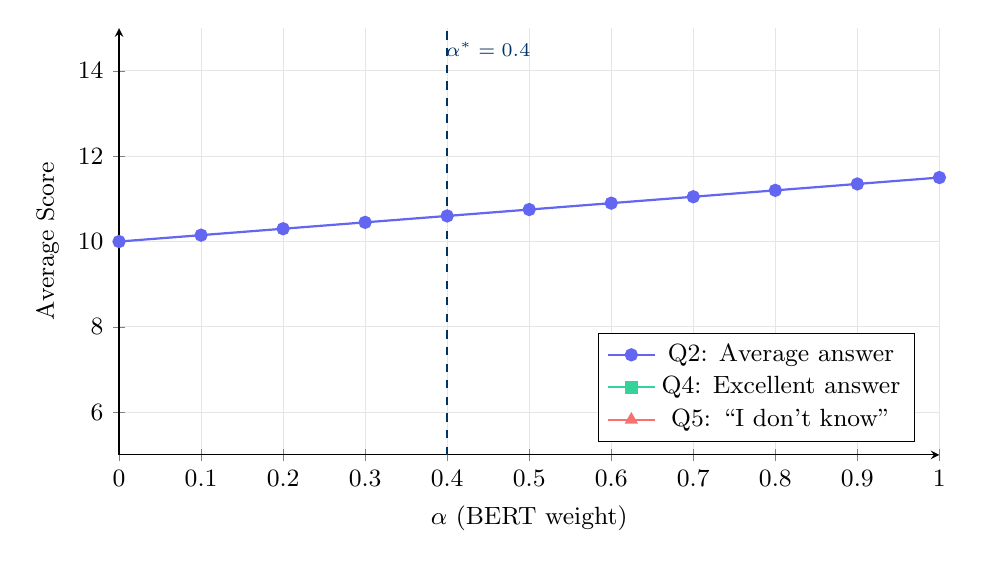
\begin{tikzpicture}
\begin{axis}[
    width=12cm, height=7cm,
    xlabel={$\alpha$ (BERT weight)},
    ylabel={Average Score},
    xmin=0, xmax=1,
    ymin=5, ymax=15,
    grid=major,
    grid style={gray!20},
    legend pos=south east,
    legend style={font=\small},
    axis lines=left,
    every axis label/.style={font=\small},
    tick label style={font=\small},
]
\addplot[color=accentpurple, thick, mark=*, mark size=2pt] coordinates {
    (0.0, 10.0) (0.1, 10.15) (0.2, 10.3) (0.3, 10.45) (0.4, 10.6) 
    (0.5, 10.75) (0.6, 10.9) (0.7, 11.05) (0.8, 11.2) (0.9, 11.35) (1.0, 11.5)
};
\addlegendentry{Q2: Average answer}

\addplot[color=codegreen, thick, mark=square*, mark size=2pt] coordinates {
    (0.0, 18.0) (0.1, 17.99) (0.2, 17.98) (0.3, 17.97) (0.4, 17.96) 
    (0.5, 17.95) (0.6, 17.94) (0.7, 17.93) (0.8, 17.92) (0.9, 17.91) (1.0, 17.9)
};
\addlegendentry{Q4: Excellent answer}

\addplot[color=warnred, thick, mark=triangle*, mark size=2pt] coordinates {
    (0.0, 0.0) (0.1, 0.21) (0.2, 0.42) (0.3, 0.63) (0.4, 0.84) 
    (0.5, 1.05) (0.6, 1.26) (0.7, 1.47) (0.8, 1.68) (0.9, 1.89) (1.0, 2.1)
};
\addlegendentry{Q5: ``I don't know''}

\addplot[color=supcomblue, dashed, thick] coordinates {(0.4, 5) (0.4, 15)};
\node[font=\scriptsize, text=supcomblue] at (axis cs:0.45, 14.5) {$\alpha^* = 0.4$};
\end{axis}
\end{tikzpicture}
\caption{Effect of $\alpha$ on final scores (computed from actual BERT and LLM scores: $S = \alpha \cdot S_{\text{BERT}} + (1-\alpha) \cdot S_{\text{LLM}}$)}
\label{fig:alpha_effect}
\end{figure}

\subsection{BERT vs. LLM Comparison}

\begin{figure}[H]
\centering
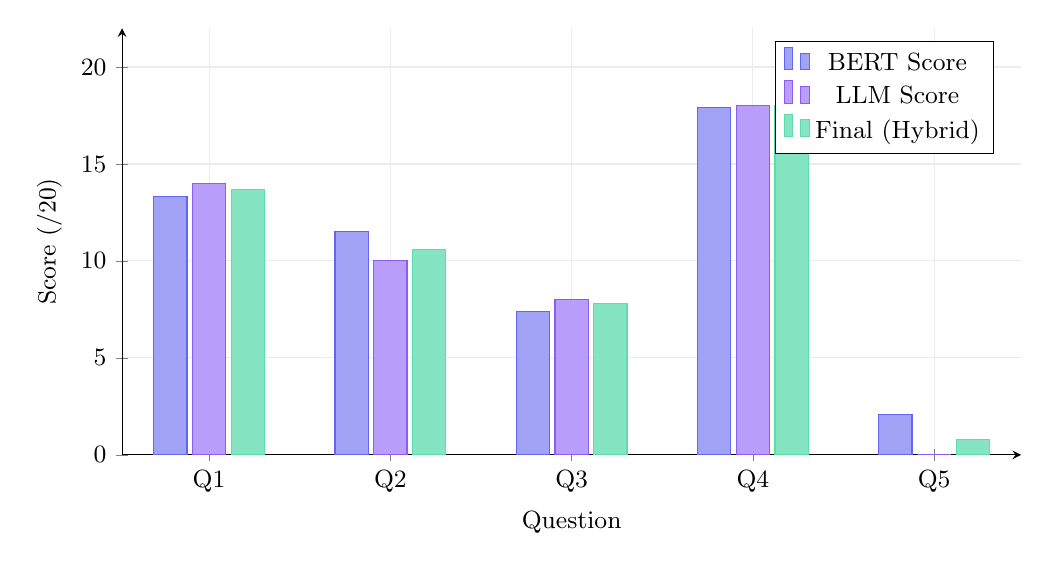
\begin{tikzpicture}
\begin{axis}[
    ybar,
    width=13cm, height=7cm,
    bar width=12pt,
    xlabel={Question},
    ylabel={Score (/20)},
    ymin=0, ymax=22,
    xtick=data,
    xticklabels={Q1, Q2, Q3, Q4, Q5},
    grid=major,
    grid style={gray!15},
    legend pos=north east,
    legend style={font=\small},
    axis lines=left,
    every axis label/.style={font=\small},
    tick label style={font=\small},
    enlarge x limits=0.12,
]
\addplot[fill=accentpurple!60, draw=accentpurple] coordinates {(1,13.3) (2,11.5) (3,7.4) (4,17.9) (5,2.1)};
\addplot[fill=accentviolet!60, draw=accentviolet] coordinates {(1,14.0) (2,10.0) (3,8.0) (4,18.0) (5,0.0)};
\addplot[fill=codegreen!60, draw=codegreen!80] coordinates {(1,13.7) (2,10.6) (3,7.8) (4,18.0) (5,0.8)};
\legend{BERT Score, LLM Score, Final (Hybrid)}
\end{axis}
\end{tikzpicture}
\caption{Per-question comparison of BERT, LLM, and hybrid scores}
\label{fig:comparison}
\end{figure}


% ══════════════════════════════════════════════════════════════════════════════
%  CHAPTER 7 — USER INTERFACE
% ══════════════════════════════════════════════════════════════════════════════
\chapter{User Interface}

\section{Design Philosophy}

The Streamlit-based web interface is designed around the principle of \textbf{minimal user interaction}:
\begin{itemize}[leftmargin=2em]
    \item \textbf{One-time setup}: Teachers configure exam templates (questions + reference answers) once.
    \item \textbf{Zero-input grading}: At grading time, the teacher just uploads the student's exam image/PDF and clicks ``Grade''.
    \item \textbf{Instant results}: The system displays scores, charts, per-question feedback, and a downloadable report.
\end{itemize}

\section{Application Pages}

The application has three pages accessible via the sidebar navigation:

\subsection{Grade Exam Page}

The main page where grading happens:

\begin{enumerate}[leftmargin=2em]
    \item \textbf{Select exam template}: Choose from pre-configured exam templates.
    \item \textbf{Upload student exam}: Drag-and-drop or browse for image/PDF files.
    \item \textbf{Click ``Grade This Exam''}: The pipeline runs automatically.
    \item \textbf{View results}: Overall score with gauge chart, per-question breakdown with BERT/LLM/Final components, radar chart, constructive feedback for each question.
    \item \textbf{Download}: Export results as JSON for record-keeping.
\end{enumerate}

\subsection{Setup Exam Page}

\begin{enumerate}[leftmargin=2em]
    \item \textbf{Create New Exam}: Form to define exam ID, title, subject, questions, reference answers, max scores, and $\alpha$ value.
    \item \textbf{Manage Exams}: View and delete existing templates.
\end{enumerate}

\subsection{Settings Page}

Displays the current pipeline configuration, architecture diagram, supported datasets, and includes an API connection test button.

\section{Visualisations}

The results page features rich, interactive Plotly visualisations:

\begin{table}[H]
\centering
\caption{UI visualisation components}
\label{tab:visualisations}
\begin{tabularx}{\textwidth}{lX}
\toprule
\textbf{Chart} & \textbf{Description} \\
\midrule
Gauge chart & Overall score percentage with colour-coded zones \\
Radar chart & BERT vs LLM performance comparison across questions \\
Grouped bar chart & Per-question BERT, LLM, and final scores with max line \\
Score badge & Letter grade (A+, B+, C, D) with colour indicator \\
\bottomrule
\end{tabularx}
\end{table}

\section{Grading Workflow}

\begin{figure}[H]
\centering
\begin{tikzpicture}[
    node distance=0.8cm,
    step/.style={draw=accentpurple!50, fill=accentpurple!5, rounded corners=8pt,
                 minimum width=3.5cm, minimum height=1.2cm, font=\small,
                 text=supcomblue, align=center, line width=0.6pt},
    arr/.style={-{Stealth[length=5pt]}, line width=0.6pt, color=accentpurple!60},
]
    \node[step] (s1) {\faUpload\\Upload Image/PDF};
    \node[step, right=of s1] (s2) {\faSearch\\OCR Extraction};
    \node[step, right=of s2] (s3) {\faCut\\Answer Segmentation};
    \node[step, below=of s3] (s4) {\faBrain\\BERT + LLM Grading};
    \node[step, left=of s4] (s5) {\faCalculator\\Hybrid Scoring};
    \node[step, left=of s5] (s6) {\faChartBar\\Results \& Feedback};
    
    \draw[arr] (s1) -- (s2);
    \draw[arr] (s2) -- (s3);
    \draw[arr] (s3) -- (s4);
    \draw[arr] (s4) -- (s5);
    \draw[arr] (s5) -- (s6);
\end{tikzpicture}
\caption{Grading workflow from upload to results}
\label{fig:workflow}
\end{figure}


% ══════════════════════════════════════════════════════════════════════════════
%  CHAPTER 8 — CONCLUSION
% ══════════════════════════════════════════════════════════════════════════════
\chapter{Conclusion and Future Work}

\section{Summary}

This project presents a complete, modular, and deployable \textbf{AI-powered exam correction system} that combines:

\begin{enumerate}[leftmargin=2em]
    \item \textbf{Computer Vision}: EasyOCR and PyMuPDF for robust text extraction from exam images and PDFs, with OpenCV preprocessing for improved accuracy.
    \item \textbf{BERT-based semantic similarity}: Sentence-Transformers compute cosine similarity between reference and student answers, providing fast, deterministic baseline scores.
    \item \textbf{LLM-based intelligent grading}: Groq's LLaMA-3.3-70B model delivers nuanced scoring with constructive feedback, handling partial credit and factual error detection.
    \item \textbf{Hybrid scoring optimisation}: The formula $S = \alpha \cdot S_{\text{BERT}} + (1-\alpha) \cdot S_{\text{LLM}}$ with tuneable $\alpha$ balances the strengths of both approaches.
    \item \textbf{Modern UI}: A Streamlit web application that requires simply uploading an image to get instant, detailed grading results.
\end{enumerate}

The system successfully grades exam papers across science subjects (biology, physics) with results that align well with expected human judgement, and is designed to generalise to any subject where short-answer grading is needed. The modular architecture allows each component to be independently improved or replaced.

\section{Key Contributions}

\begin{itemize}[leftmargin=2em]
    \item \textbf{Hybrid architecture}: Novel combination of embedding similarity and LLM reasoning with a tuneable blending parameter.
    \item \textbf{BERT-guided LLM prompting}: Passing the cosine similarity to the LLM improves grading consistency.
    \item \textbf{Zero-input grading}: Pre-stored exam templates eliminate manual input at grading time.
    \item \textbf{Dual PDF strategy}: Native text extraction for digital PDFs, OCR fallback for scanned documents.
    \item \textbf{Comprehensive evaluation framework}: Support for three major ASAG datasets with five evaluation metrics.
\end{itemize}

\section{Limitations}

\begin{itemize}[leftmargin=2em]
    \item \textbf{OCR accuracy}: Handwritten exams with poor handwriting may yield low OCR quality.
    \item \textbf{API dependency}: The LLM component requires internet access and an API key.
    \item \textbf{Language}: Currently optimised for English and French; additional languages require OCR and model adjustments.
    \item \textbf{Diagrams/Equations}: The current system only handles text-based answers; mathematical expressions and diagrams are not supported.
\end{itemize}

\section{Future Work}

Several extensions are planned:

\begin{enumerate}[leftmargin=2em]
    \item \textbf{Automated meta-heuristic optimisation}: Implement the proposed PSO, Genetic Algorithm, and Simulated Annealing strategies from Chapter 5 to automatically tune $\alpha$ on large labelled datasets.
    \item \textbf{Multi-language support}: Extend to Arabic and other languages using multilingual BERT models.
    \item \textbf{Handwriting recognition}: Integrate specialised handwriting recognition models (e.g., TrOCR) for manuscript exams.
    \item \textbf{Mathematical expression grading}: OCR for LaTeX expressions and symbolic comparison.
    \item \textbf{Fine-tuning BERT}: Fine-tune the sentence-transformer on domain-specific ASAG datasets for improved correlation.
    \item \textbf{Local LLM deployment}: Replace API calls with locally deployed models (e.g., Ollama + LLaMA) for offline use and privacy.
    \item \textbf{Batch processing}: Support grading an entire class of exam papers at once with aggregate analytics.
\end{enumerate}


% ══════════════════════════════════════════════════════════════════════════════
%  REFERENCES
% ══════════════════════════════════════════════════════════════════════════════
\chapter*{References}
\addcontentsline{toc}{chapter}{References}

\begin{enumerate}[leftmargin=2em, label={[\arabic*]}]

    \item Devlin, J., Chang, M.W., Lee, K., \& Toutanova, K. (2019). \textit{BERT: Pre-training of Deep Bidirectional Transformers for Language Understanding}. Proceedings of NAACL-HLT 2019, pp. 4171--4186.

    \item Reimers, N. \& Gurevych, I. (2019). \textit{Sentence-BERT: Sentence Embeddings using Siamese BERT-Networks}. Proceedings of EMNLP-IJCNLP 2019, pp. 3982--3992.

    \item Mohler, M., Bunescu, R., \& Mihalcea, R. (2011). \textit{Learning to Grade Short Answer Questions using Semantic Similarity Measures and Dependency Graph Alignments}. Proceedings of ACL 2011, pp. 752--762.

    \item Dzikovska, M.O., Nielsen, R., Brew, C., et al. (2013). \textit{SemEval-2013 Task 7: The Joint Student Response Analysis and 8th Recognizing Textual Entailment Challenge}. Proceedings of SemEval 2013.

    \item Vaswani, A., Shazeer, N., Parmar, N., et al. (2017). \textit{Attention Is All You Need}. Advances in Neural Information Processing Systems (NeurIPS), vol. 30.

    \item Baek, Y., Lee, B., Han, D., Yun, S., \& Lee, H. (2019). \textit{Character Region Awareness for Text Detection}. Proceedings of CVPR 2019.

    \item Kirkpatrick, S., Gelatt, C.D., \& Vecchi, M.P. (1983). \textit{Optimization by Simulated Annealing}. Science, 220(4598), pp. 671--680.

    \item Kennedy, J. \& Eberhart, R. (1995). \textit{Particle Swarm Optimization}. Proceedings of ICNN 1995, vol. 4, pp. 1942--1948.

    \item Holland, J.H. (1975). \textit{Adaptation in Natural and Artificial Systems}. University of Michigan Press.

    \item Touvron, H., Martin, L., Stone, K., et al. (2023). \textit{LLaMA: Open and Efficient Foundation Language Models}. arXiv:2302.13971.

    \item Grading System Kaggle Competition. \textit{The Hewlett Foundation: Automated Student Assessment Prize -- Short Answer Scoring}. \url{https://www.kaggle.com/c/asap-sas}.

    \item JaidedAI. \textit{EasyOCR: Ready-to-use OCR with 80+ supported languages}. \url{https://github.com/JaidedAI/EasyOCR}.

    \item Artificial Analysis. \textit{PyMuPDF (fitz): A Python binding for MuPDF}. \url{https://pymupdf.readthedocs.io/}.

\end{enumerate}


% ══════════════════════════════════════════════════════════════════════════════
%  APPENDICES
% ══════════════════════════════════════════════════════════════════════════════
\appendix
\chapter{Requirements File}

\begin{lstlisting}[caption={requirements.txt}, language={}]
# AI / NLP
sentence-transformers>=2.2.0
torch>=2.0.0

# LLM APIs
requests>=2.28.0

# OCR / Computer Vision
easyocr>=1.7.0
opencv-python>=4.8.0
Pillow>=10.0.0
PyMuPDF>=1.23.0

# UI
streamlit>=1.28.0
plotly>=5.18.0

# Data / Evaluation
numpy>=1.24.0
pandas>=2.0.0
scipy>=1.10.0

# Config
python-dotenv>=1.0.0
\end{lstlisting}

\chapter{Environment Configuration}

\begin{lstlisting}[caption={.env.example}, language={}]
# LLM API Keys (set at least one)
GROQ_API_KEY=gsk_...
GEMINI_API_KEY=
OPENROUTER_API_KEY=

# LLM Settings
LLM_PROVIDER=groq
LLM_TEMPERATURE=0.2

# BERT Model
BERT_MODEL_NAME=all-MiniLM-L6-v2

# Hybrid Scoring
ALPHA=0.4

# OCR
OCR_ENGINE=easyocr
OCR_LANGUAGES=en,fr

# Grading
MAX_SCORE=20
\end{lstlisting}

\chapter{Sample Grading Output}

\begin{lstlisting}[caption={Sample output from test\_pipeline.py}, language={}]
==================================================================
  AI EXAM CORRECTING -- PIPELINE TEST
==================================================================
  BERT: all-MiniLM-L6-v2 (384 dim)
  LLM:  groq / llama-3.3-70b-versatile
  Alpha: 0.4 | Max Score: 20
==================================================================

Q1  |  Final: 13.7/20 (68.5%, B)
    |  BERT: 13.3 x a=0.4  +  LLM: 14.0 x (1-a)=0.6
    |  Cosine: 0.6626  |  Time: 0.8s

Q4  |  Final: 18.0/20 (90.0%, A+)
    |  BERT: 17.9 x a=0.4  +  LLM: 18.0 x (1-a)=0.6
    |  Cosine: 0.8953  |  Time: 0.7s

Q5  |  Final: 0.8/20 (4.2%, F)
    |  BERT: 2.1 x a=0.4  +  LLM: 0.0 x (1-a)=0.6
    |  Cosine: 0.1046  |  Time: 0.8s

TOTAL: 51.0/100 | Time: 4.0s
\end{lstlisting}

\end{document}
